\documentclass[12pt,a4paper]{article}

\usepackage{inputenc}
\usepackage[british,UKenglish]{babel}
\usepackage{amsmath}
%\usepackage{titlesec}
\usepackage{color}
\usepackage{graphicx}
\usepackage{fancyref}
\usepackage{hyperref}
\usepackage{float}
\usepackage{scrextend}
\usepackage{setspace}
\usepackage{xargs}
\usepackage{multicol}
\usepackage{nameref}

\usepackage{sectsty}
\usepackage{multicol}
\usepackage{multirow}
\usepackage[procnames]{listings}
\usepackage{appendix}
\usepackage{geometry}
\usepackage{titlesec}

\newcommand\tab[1][1cm]{\hspace*{#1}}
\hypersetup{colorlinks=true, linkcolor=black}
\interfootnotelinepenalty=10000

\newcommand{\cleancode}[1]{\begin{addmargin}[3em]{3em}\texttt{\textcolor{cleanOrange}{#1}}\end{addmargin}}
\newcommand{\cleanstyle}[1]{\text{\textcolor{cleanOrange}{\texttt{#1}}}}


\usepackage[colorinlistoftodos,prependcaption,textsize=footnotesize]{todonotes}
\newcommandx{\commred}[2][1=]{\textcolor{Red}
{\todo[linecolor=red,backgroundcolor=red!25,bordercolor=red,#1]{#2}}}
\newcommandx{\commblue}[2][1=]{\textcolor{Blue}
{\todo[linecolor=blue,backgroundcolor=blue!25,bordercolor=blue,#1]{#2}}}
\newcommandx{\commgreen}[2][1=]{\textcolor{OliveGreen}{\todo[linecolor=OliveGreen,backgroundcolor=OliveGreen!25,bordercolor=OliveGreen,#1]{#2}}}
\newcommandx{\commpurp}[2][1=]{\textcolor{Plum}{\todo[linecolor=Plum,backgroundcolor=Plum!25,bordercolor=Plum,#1]{#2}}}

\def\code#1{{\tt #1}}

\def\note#1{\noindent{\bf [Note: #1]}}

\makeatletter
%% The "\@seccntformat" command is an auxiliary command
%% (see pp. 26f. of 'The LaTeX Companion,' 2nd. ed.)
\def\@seccntformat#1{\@ifundefined{#1@cntformat}%
   {\csname the#1\endcsname\quad}  % default
   {\csname #1@cntformat\endcsname}% enable individual control
}
\let\oldappendix\appendix %% save current definition of \appendix
\renewcommand\appendix{%
    \oldappendix
    \newcommand{\section@cntformat}{\appendixname~\thesection\quad}
}
\makeatother


% "define" Scala
\usepackage[T1]{fontenc}  
\usepackage[scaled=0.82]{beramono}  
\usepackage{microtype} 

\sbox0{\small\ttfamily A}
\edef\mybasewidth{\the\wd0 }

\lstdefinelanguage{scala}{
  morekeywords={abstract,case,catch,class,def,%
    do,else,extends,false,final,finally,%
    for,if,implicit,import,match,mixin,%
    new,null,object,override,package,%
    private,protected,requires,return,sealed,%
    super,this,throw,trait,true,try,%
    type,val,var,while,with,yield},
  sensitive=true,
  morecomment=[l]{//},
  morecomment=[n]{/*}{*/},
  morestring=[b]",
  morestring=[b]',
  morestring=[b]"""
}

\usepackage{color}
\definecolor{dkgreen}{rgb}{0,0.6,0}
\definecolor{gray}{rgb}{0.5,0.5,0.5}
\definecolor{mauve}{rgb}{0.58,0,0.82}

% Default settings for code listings
\lstset{frame=tb,
  language=scala,
  aboveskip=3mm,
  belowskip=3mm,
  showstringspaces=false,
  columns=fixed, % basewidth=\mybasewidth,
  basicstyle={\small\ttfamily},
  numbers=none,
  numberstyle=\footnotesize\color{gray},
  % identifierstyle=\color{red},
  keywordstyle=\color{blue},
  commentstyle=\color{dkgreen},
  stringstyle=\color{mauve},
  frame=single,
  breaklines=true,
  breakatwhitespace=true,
  procnamekeys={def, val, var, class, trait, object, extends},
  procnamestyle=\ttfamily\color{red},
  tabsize=2
}

\lstnewenvironment{scala}[1][]
{\lstset{language=scala,#1}}
{}
\lstnewenvironment{cpp}[1][]
{\lstset{language=C++,#1}}
{}
\lstnewenvironment{bash}[1][]
{\lstset{language=bash,#1}}
{}
\lstnewenvironment{verilog}[1][]
{\lstset{language=verilog,#1}}
{}



\lstset{frame=, basicstyle={\footnotesize\ttfamily}}
\geometry{left=3.17cm,right=3.17cm,top=2.54cm,bottom=2.54cm}
% 常规页眉页脚
\newpagestyle{main}{            
    \sethead{}{}{}     %设置页眉
    \setfoot{}{\thepage}{}      %设置页脚,可以在页脚添加 \thepage  显示页数
    \headrule                                      % 添加页眉的下划线
    \footrule                                       %添加页脚的下划线
}

% 封面页眉页脚
\newpagestyle{title}{            
    \sethead{报告号: 774323540--10dz1200500/01}{}{}     %设置页眉
%    \setfoot{左页脚}{\thepage}{右页脚}      %设置页脚,可以在页脚添加 \thepage  显示页数
    \headrule                                      % 添加页眉的下划线
    \footrule                                       %添加页脚的下划线
}

\pagestyle{main}

\graphicspath{ {images/} }
\usepackage{ctex}
\usepackage{caption}
\usepackage{subfigure}
\usepackage{booktabs}
\usepackage{amsthm}

\theoremstyle{definition}
\newtheorem{definition}{Definition}[section]
\newtheorem{lemma}{Lemma}
%-----------------------------------------BEGIN DOC----------------------------------------

\begin{document}
\renewcommand{\contentsname}{\ \ \ 目录\ \ \ }
\renewcommand{\appendixname}{附录}
\renewcommand{\appendixpagename}{附录}
\renewcommand{\refname}{参考文献} 
\renewcommand{\figurename}{图}
\renewcommand{\tablename}{表}
\renewcommand{\today}{\number\year 年 \number\month 月 \number\day 日}

\renewcommand{\maketitle}{
    \thispagestyle{title}
    \heiti
    \vspace*{94pt}
    \begin{center}
        \fontsize{50pt}{0} 科技报告\\
        \vspace*{300pt}
        \large \textcolor{red}{报告名称: \quad}\ \ \underline{\makebox[300pt]{陈家镇国际生态社区能源管理中心建设关键技术}}\\
        \large 支持渠道: \quad\ \ \underline{\makebox[300pt]{科技部等中央单位与上海市共同推进重大任务科研专项}}\\
        \large 报告类型: \quad\ \ \underline{\makebox[300pt]{最终报告}}\\
        \large 编制单位: \quad\ \ \underline{\makebox[300pt]{上海陈家镇建设发展有限公司}}\\
        \large 编制时间: \quad\ \ \underline{\makebox[300pt]{\today}}

    \end{center}
}

\maketitle

\newpage

%-----------------------------------------ABSTRACT-------------------------------------
\begin{center}
{\Large\bf{摘\ 要\\}}
\end{center}
请在这里输入摘要内容.
\newpage
%-----------------------------------------ABSTRACT-------------------------------------
\begin{center}
{\Large\bf{版\ 权\ 声\ 明\\}}
\end{center}
该文件受《中华人名共和国著作权法》的保护。ERCESI实验室保留拒绝授权违法复制该文件的权利。任何收存和保管本文件各种版本的单位和个人,未经ERCESI实验室(西北工业大学)同意,不得将本文档转借他人,亦不得随意复制、抄录、拍照或以任何方式传播。 否则,引起有碍著作权之问题,将可能承担法律责任。\newpage
%-----------------------------------------CONTENT-------------------------------------
\begin{center}
\tableofcontents\label{c}
\end{center}

%------------------------------------------TEXT--------------------------------------------

%----------------------------------------OVERVIEW-----------------------------------------

%----------------------------------SYSTEM DESIGN------------------------------------------

% -----------------------------------BLOCKS DESIGN----------------------------------------

\newpage
\section{技术背景}\label{Background}

\newpage
\section{微服务动态演化一致性保障协议}\label{section:version_consistency}

\subsection{基本原理}
本小节将阐述微服务动态演化一致性保障协议的基本原理,说明如何保证正确且高效地完成系统的动态演化。首先引入一个简单但又不失一般性的例子,在系统中存在着这样四个微服务:Portal、Proc、Auth和DB。用户首先会向Portal微服务发起请求,收到请求后的Portal微服务先是调用Auth微服务,得到当前请求的一个验证令牌。然后Portal使用得到的令牌接着对Proc微服务发起请求,收到请求的Proc微服务利用随请求而来的令牌向Auth微服务进行验证,若收到的回复是验证通过,则进一步调用DB微服务以读取数据库中的具体信息并返回;否则,返回请求失败消息,然后将最终结果反馈给发起请求的用户。
\begin{figure}[ht]
 \centering
 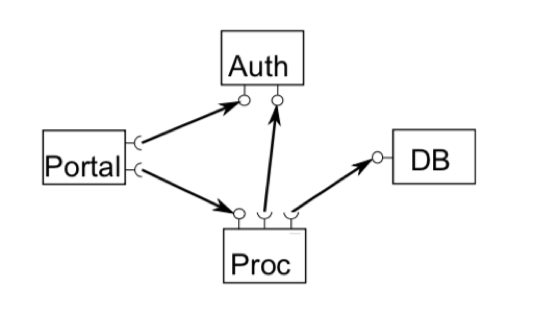
\includegraphics[height=5cm]{images/Example.png}
 \caption{示例系统}
 \label{fig:Example}
\end{figure}


考虑到这样一种情况:在系统运行时,由于采用了更为安全和快速的加解密算法,由于整个系统所有的加解密过程都在Auth微服务中进行,因此我们可以仅对Auth微服务进行版本的更新及替换,同时对其它的微服务保持透明。在前述的系统运行流程中,若我们在Portal微服务调用完Auth微服务得到对应的验证令牌后且Proc微服务还未使用该令牌向Auth微服务发起验证之前的这个时间段内,Auth微服务不服务于任何的事务,处于空闲状态,我们对Auth微服务进行版本的更新及替换。随着系统的继续运行,当Proc微服务利用使用旧版本算法所加密生成的验证令牌来向Auth微服务发起调用,但此时的Auth微服务已完成更新,新旧算法的不兼容性导致验证失败,最终返回失败信息。显然Auth微服务不正确的动态演化,导致了系统在无故障的情况下不能正确地处理用户请求。

动态演化要求系统能够在不停止服务的情况下进行更新,用户发出的请求在更新前后都能被正确地处理且返回结果。因此,微服务动态演化一致性保障协议的基本原理是考虑在系统运行的过程中,当一次请求需要多次涉及同一个微服务,且不同版本的微服务因兼容性等原因将返回不同的结果时,需要依据事务的运行流程来决定调用的服务版本,从而保证用户请求不受服务动态演化的影响。

\subsection{一致性保障协议}
在介绍一致性保障协议之前,首先介绍协议中将要用到的几个基本概念的定义:

\theoremstyle{definition}
\begin{definition}[\textbf{事务与分布式事务}]
\label{definition:transaction}
\textbf{一个事务表示在某一微服务上执行且在有限时间内结束的一系列操作,操作包括本地数据的计算和微服务间消息的传递等。在某一微服务上运行的事务可以向其它微服务发起请求,从而在其它的微服务中生成一个新的事务。前者和后者之间的事务关系我们称为父子事务,外界调用系统所产生的第一个事务为根事务。根事务及其随后的调用所产生的所有子事务,我们称为一个分布式事务,并使用其根事务的符号进行标识。}
\end{definition}

\begin{figure}[ht]
 \centering
 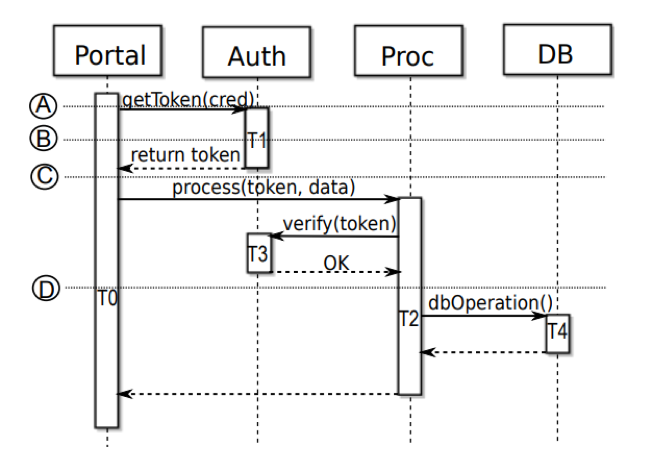
\includegraphics[height=8cm]{images/ExampleProcess.png}
 \caption{示例系统运行时序图}
 \label{fig:ExampleProcess}
\end{figure}


上图即表示了我们前面所描述的系统中四个微服务之间的运行流程。外部请求首先在Portal微服务上生成T0根事务,然后通过微服务间的调用T1、T2、T3、T4事务依次生成。这样一次完整的调用过程我们便称为分布式事务,用根事务符号T0来进行表示,而T1~T4事务都可称为是T0的子事务。

\begin{definition}[\textbf{版本一致性}]
\label{definition:version_consistency}
\textbf{一个分布式事务是版本一致的,当且仅当不存在它的两个子事务,它们在系统运行时先后在同一个微服务的不同版本上运行。一次动态演化所导致的系统演化是版本一致的,当且仅当所有的分布式事务是版本一致的。}
\end{definition}



在我们前面所描述的系统运行的例子中,考虑对Auth微服务进行更新,如果更新发生在根事务T0生成之后,但在生成T1之前(即时刻A),那么后续在Auth微服务上生成的T1、T3子事务都使用的是Auth微服务的新版本,分布式事务T0满足版本一致性;如果更新发生在T3子事务完成之后(即时刻D),那么在Auth微服务执行过的T1、T3子事务都使用的是Auth微服务的旧版本,分布式事务T0满足版本一致性;而在前面系统出现错误的例子中,更新发生在子事务T1完成之后, 但T2子事务还未生成之前(即时刻C),那么将导致T1子事务和T3子事务在Auth微服务的不同版本上运行,此时分布式事务T0便不满足版本一致性。

版本一致性虽然描述了微服务动态演化的准则,但我们并不能直接利用这个规则来对微服务动态演化的时机进行判断,因此我们需要引入动态依赖边,使得我们可以分布式地在各自的微服务上进行本地的操作,便可以判断当前微服务是否满足动态演化的条件(即版本一致性)。

\begin{definition}[\textbf{动态依赖边}]
\label{definition:dynamic_dependences}
\textbf{$C \xrightarrow[T]{future(past)}  C'$表示在分布式事务T的运行过程中,有一条从微服务C到微服务$C'$的future(past)边。
其中,future边表示在T之后的运行过程中,微服务C有可能还会在微服务$C'$上生成新的子事务;past边表示在T之前的运行过程中,微服务C已经在微服务$C'$上成功地生成过子事务并返回。}
\end{definition}



有了动态依赖边的定义,我们使用如下的规范性准则,使得依赖边可以在每一个分布式事务的运行过程中动态且正确地进行增加和删除操作:

\begin{itemize}
\item{在微服务C上运行的每一个事务T,开始时添加一对动态依赖边( $C \xrightarrow[root(T)]{future}C$ 和 $C \xrightarrow[root(T)]{past}C$ ),标识为T的根事务,事务结束时删除;}


\item{每一条动态依赖边,都需要微服务C和微服务$C'$之间存在真正的静态边,即存在对应调用关系;}


\item{$C \xrightarrow[T]{future}C'$ 边必须要在T的第一个子事务生成之前添加,并且应等到T不会通过微服务C在微服务$C'$上生成子事务时,才能够删除;}


\item{$C \xrightarrow[T]{past}C'$ 边在T的运行过程中,当微服务C在微服务$C'$上生成的子事务即将结束时生成,应等到T结束时才能够删除。}
\end{itemize}

有了上述动态依赖边的支持,在系统运行的任何时刻,每个微服务都可以知晓指向自己的动态依赖边,以及负责从自己指向其它微服务动态依赖边的增删,所以我们可以将动态演化的版本一致性条件转化为本地可判断的闲置(FREENESS)条件:

\begin{definition}[\textbf{闲置(FREENESS)}]
\label{definition:freeness}
\textbf{微服务C针对某一个分布式事务T是版本一致的,当且仅当不存在由T标识的一对future/past边指向微服务C。微服务C在某一时刻下的状态是版本一致的,当且仅当微服务C对所有当前运行的分布式事务是版本一致的。}
\end{definition}


\subsection{微服务动态演化过程}
利用动态依赖边的定义以及增删的规范性准则,带有动态依赖边的分布式事务T在运行时流程具体表现为如下三个阶段:

\begin{enumerate}

\item [1.] 准备阶段:分布式事务T在第一个微服务C上完成初始化但还未调用任何其它微服务,即生成子事务之前,C通知所有可能依赖的微服务创建future边并等待回复。被通知的微服务同理,通知其依赖的微服务执行创建操作。当收到所有future边创建成功的回复后,事务T开始运行,如图\ref{fig:Process_a};
\begin{figure}[ht]
 \centering
 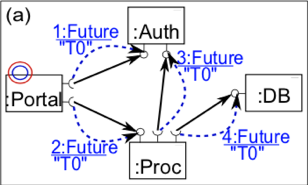
\includegraphics[height=5cm]{images/Process_a.png}
 \caption{准备阶段:process\_a}
 \label{fig:Process_a}
\end{figure}


\item [2.] 运行阶段:当知道微服务C不会再通过静态边 $C \xrightarrow{static}C'$ 在微服务C’上生成T的子事务,而且不存在指向C的标识为T的future边,那么future边 $C \xrightarrow[T]{future}C'$ 可以被删除;当微服务$C'$上标识为T的子事务将要结束时,通知微服务C创建past边 $C \xrightarrow[T]{past}C'$ ,且应保证创建成功才能结束子事务,如图\ref{fig:process_c and process_d};
\begin{figure}[htbp]
\centering
\begin{minipage}[t]{0.48\textwidth}
\centering
\centerline{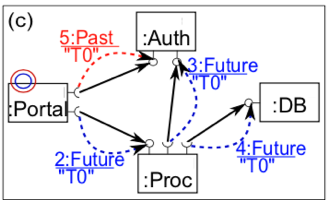
\includegraphics[width=6cm]{Process_c.png}}
\label{fig:process_c}
\end{minipage}
\begin{minipage}[t]{0.48\textwidth}
\centering
\centerline{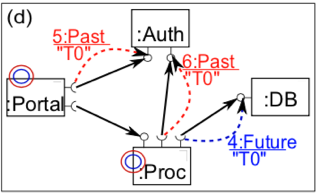
\includegraphics[width=6cm]{Process_d.png}}
\label{fig:process_d}
\end{minipage}
\caption{运行阶段:procss\_c 和 process\_d}
\label{fig:process_c and process_d}
\end{figure}


\item [3.] 结束阶段:和准备阶段时的创建操作类似,从第一个微服务C递归向所有的依赖微服务发送删除消息,删除标识为当前分布式事务T的所有动态依赖边。
\end{enumerate}

前面的运行流程中,假设我们需要对Auth微服务进行一致性演化且当前只有分布式事务T0处于运行状态,利用闲置(FREENESS)的定义,在时刻A和时刻D,Auth满足更新条件;而在时刻C,存在执行Auth微服务且标识为T0的一对future/past边,因此不满足更新条件。

微服务C只有满足了闲置(FREENESS)条件才能够进行动态演化,但由于系统处于持续运行且不断接收请求的状态,同一时刻存在不同的分布式事务在系统中运行,因此若仅仅通过等待然后判断的策略(WF),微服务有可能永远不能满足闲置(FREENESS)条件,从而无法及时地进行动态演化。除了WF策略,我们还可以使用下面的两种策略,使得微服务能够及时地完成动态演化操作:

\begin{itemize}

\item {CV:允许不同版本的微服务实例同时存在并提供服务

当微服务C需要进行动态演化时,启动新版本的实例并同时提供服务。当需要在微服务C上生成子事务T时,若已经有一条标识为root(T)的past边指向微服务C,那么新生成的子事务T将在旧版本的微服务实例上运行,否则在新版本的微服务实例上运行。由于事务会在有限时间内完成,因此旧版本的微服务实例上运行的事务逐渐减少为零,最终将旧版本实例从系统中移除。}

\item{BF:暂时阻塞新事务的生成

当微服务C需要进行动态演化时,若需要在其上生成新的子事务T,首先判断是否存在标识为root(T)的一条past边指向自己,若存在则子事务T可以在微服务C上生成并继续执行;不然,阻塞子事务T。旧版本的微服务实例上运行的事务会在有限时间内完成,最终微服务C将满足闲置(FREENESS)条件,此时进行版本的更新,然后恢复之前阻塞的所有事务。}
\end{itemize}

\newpage
\section{基于Istio的协议实现}\label{baseistio}
\subsection{Service Mesh与Istio}
传统的应用程序将所有功能都打包成一个独立的单元,因此也被称为单体应用。单体应用架构简单,在开发、测试和部署等方面都比较方便。但随着软件应用的发展,单体应用的弊端开始显现:不够灵活,对应用程序做任何细微的修改都需要将整个应用程序重新构建、重新部署,妨碍软件应用的持续交付;技术栈受限,开发团队的所有成员通常都必须使用相同的开发语言。因此,微服务架构应运而生。微服务架构将大型的单体应用拆分成若干个更小的服务,使得每个服务都可以独立地进行部署、升级、扩展和替换,服务间使用轻量级的通信协议进行通信(例如,同步的REST,异步的AMQP等),降低服务间耦合度的同时满足了软件程序对于快速持续集成和持续交付的需求。
\begin{figure}[ht]
 \centering
 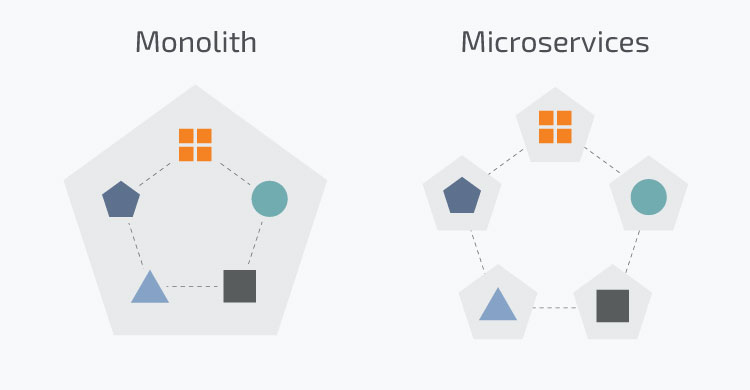
\includegraphics[height=5cm]{images/Microservices-vs-Monolith.jpg}
 \caption{单体应用和微服务应用}
 \label{fig:Microservices-vs-Monolith}
\end{figure}

与单体应用相比,微服务架构将系统应用的复杂度从单体应用内部的测试、部署、维护等转变到了微服务的连接调用、管理部署和监控等方面,因此微服务架构会极大地增加运维工作量,开发人员需要投入更多的精力来保证远程调用的可靠性与数据一致性。为了简化开发,开发人员通过典型的类库和框架(如Netflix OSS套件、Spring Cloud框架),编写较少的代码和注解就可以完成微服务间的服务发现、负载均衡、熔断、重试等功能。但此种办法缺点在于,开发人员需要掌握并熟练使用的内容较多,而且服务治理的功能不够齐全,很多功能需要自己进行拓展,编程语言也有所受限。这样所开发出来的微服务中,关键的业务逻辑代码和其它的用于管理服务间关系的非功能性代码混杂在一起。此时,若考虑为每一个微服务实例部署一个Sidecar,将所有前述的非功能性代码移到Sidecar中,由Sidecar来负责提供服务发现等辅助功能,而开发人员只需专注于微服务的业务逻辑,从而有效地进行了解耦。当为大型的微服务系统部署Sidecar时,微服务之间的服务调用关系便形成了服务网格(Service Mesh),如图\ref{fig:service_mesh}所示。
\begin{figure}[ht]
 \centering
 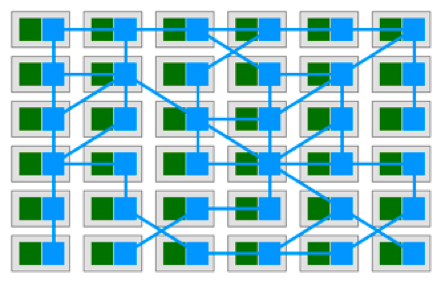
\includegraphics[height=5cm]{images/service_mesh.png}
 \caption{服务网格(Service Mesh)}
 \label{fig:service_mesh}
\end{figure}

当前最主流的Service Mesh方案,是Google和IBM两个公司联合Lyft合作的开源项目Istio。在Istio的架构中,直接在Lyft开发的Envoy之上进行了拓展,然后将其作为Sidecar代理进行部署。Envoy Proxy作为数据面,除了提供服务发现、负载均衡、限流熔断等功能,还可以协调微服务的所有出入站流量,收集相关的性能指标,与控制面进行交互。而有了数据面的支持,控制面一方面通过Pilot组件下发配置信息到相应的Envoy Proxy中,负责流量管理,另一方面通过Mixer组件收集遥测数据,从而实现了对整个微服务系统多方面的掌管与监控。
\begin{figure}[ht]
 \centering
 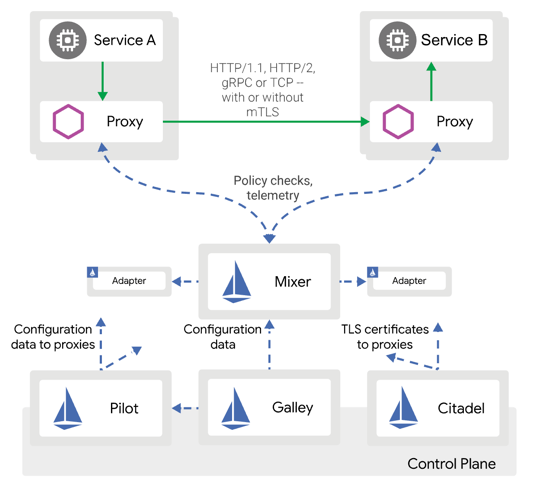
\includegraphics[height=9cm]{images/istio_arch.png}
 \caption{Istio架构图(v1.4)}
 \label{fig:istio_arch}
\end{figure}

\subsection{协议实现具体流程}
基于Istio,部署前述的示例系统,具体架构变为图\ref{fig:demo_arch_on_istio}。用户将访问请求发往Ingress Gateway,由Ingress Gateway依据相应的路由规则,再将请求转发至具体的后端服务中,然后收集运行结果并进行返回。每一次用户的请求都将产生一个分布式事务,其中可能会涉及多个服务的远程调用,但可以使用请求头中的x-b3-traceid字段进行唯一标识。Ingress Gaeway一方面将对应的服务接口暴露出来供用户进行访问,另一方面为用户屏蔽了后端服务的具体实现和路由转发等服务治理功能。

\begin{figure}[ht]
 \centering
 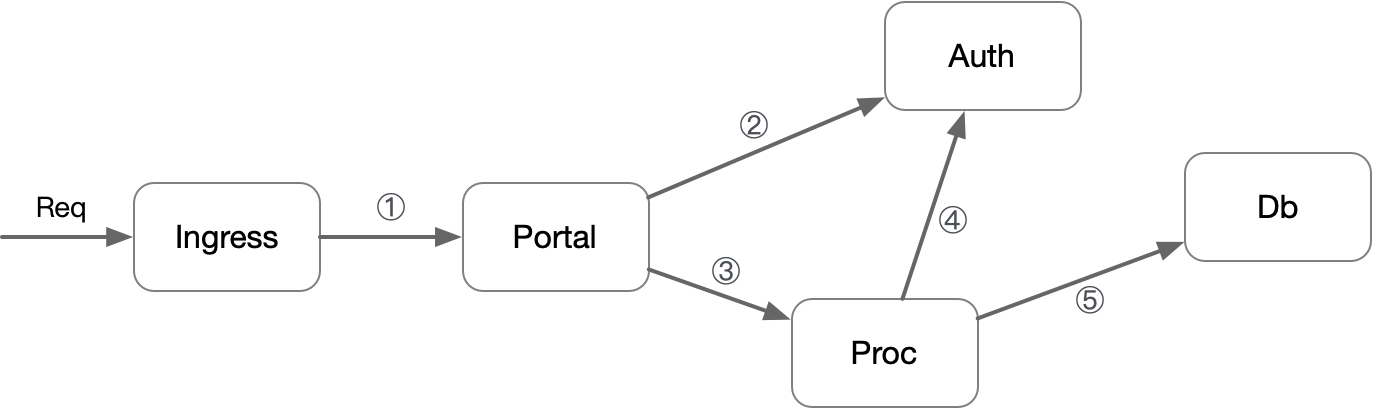
\includegraphics[height=4cm]{images/demo_arch_on_istio.png}
 \caption{Istio中的示例系统}
 \label{fig:demo_arch_on_istio}
\end{figure}

以示例系统中的auth-service服务为例,具体的实现和更新流程为:
\subsubsection{插入Envoy容器和TraceManager容器}
修改Istio框架中的自动注入功能,当每个服务实例部署时,我们将为每个服务实例对应部署Envoy容器和TraceManager容器。其中,Envoy容器负责从Istio控制面中接收用户的配置信息,然后将配置信息转换成对应的规则,对所有的出入站流量进行管理;与此同时,当存在具体的入站流量访问对应的服务时,Envoy会将此次分布式调用的唯一标识(x-b3-traceid)和相关信息发送至TraceManager中。而TraceManager容器则负责接收从Envoy容器中发送过来的信息,对其进行记录管理,为后续的更新过程提供支持。插入的Envoy和TraceManager容器分别作为客户端和服务端,通过Unix Domain Socket的方式进行通信,从而最大程度地减少了消息传送对Envoy快速处理用户请求的影响。
\begin{figure}[ht]
 \centering
 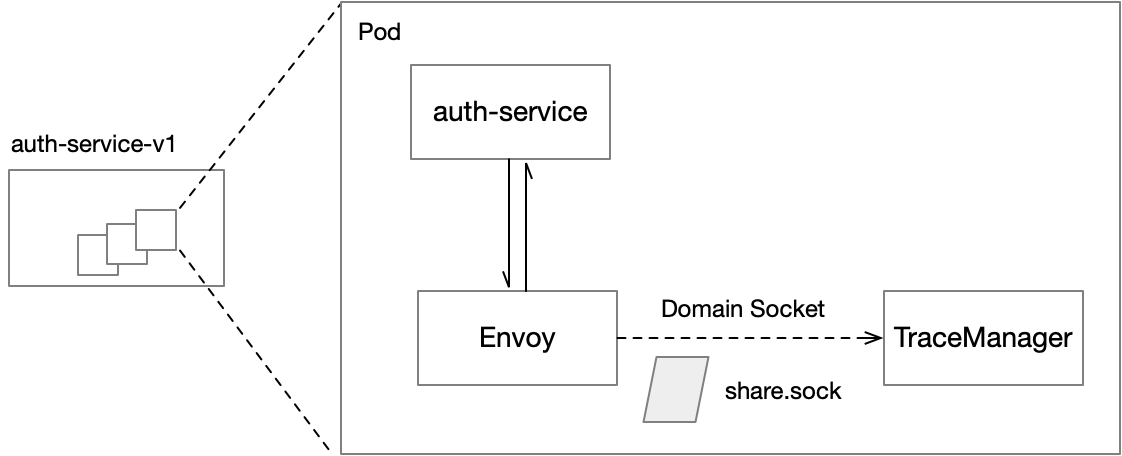
\includegraphics[height=5cm]{images/insert_containers.png}
 \caption{插入容器}
 \label{fig:insert_containers}
\end{figure}

\subsubsection{创建初始的路由规则和版本信息}\label{section:setup}当整个系统部署完成时,为每个服务创建初始的路由规则和版本信息。图\ref{fig:vs_all_v1}中定义了路由规则,要求流量调用到auth-service时,所有流量都发往v1版本,且在返回的头信息中会带上自定义的信息,后续将利用此头信息进行流量的转发;图\ref{fig:dr_v1}中定义了版本信息,说明带有{version: v1}标签的所有auth-service的服务实例都属于v1版本;此时系统的运行状态对应显示为图\ref{fig:traffic_all_v1}
\begin{figure}[htbp]
\centering
\begin{minipage}[t]{0.48\textwidth}
\centering
\centerline{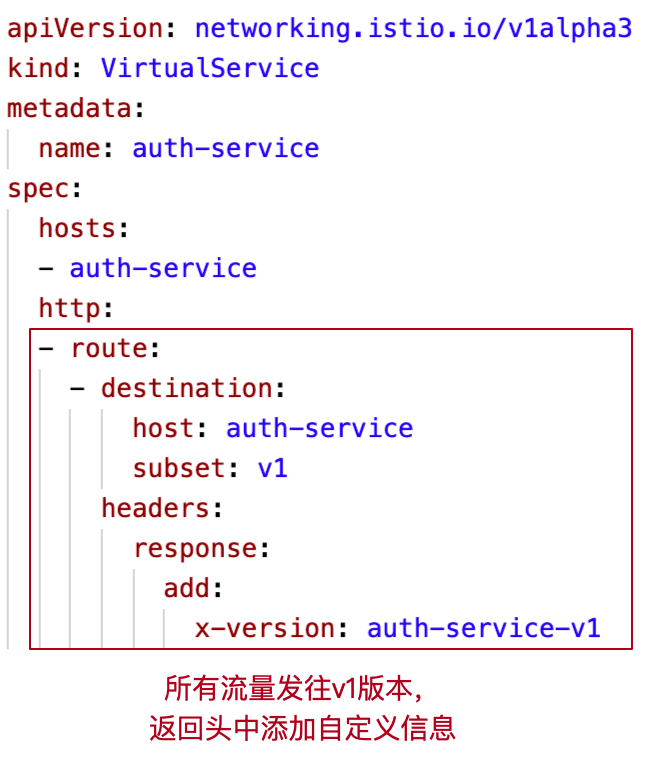
\includegraphics[width=6cm]{vs_all_v1.png}}
\caption{v1路由规则}
\label{fig:vs_all_v1}
\end{minipage}
\begin{minipage}[t]{0.48\textwidth}
\centering
\centerline{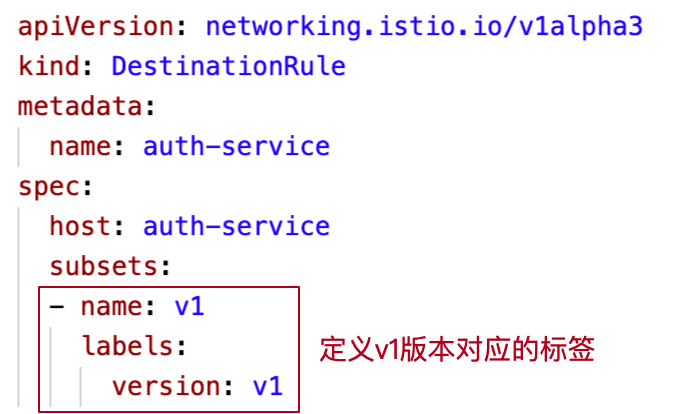
\includegraphics[width=6cm]{dr_v1.png}}
\caption{v1版本规则}
\label{fig:dr_v1}
\end{minipage}
\end{figure}

\begin{figure}[ht]
 \centering
 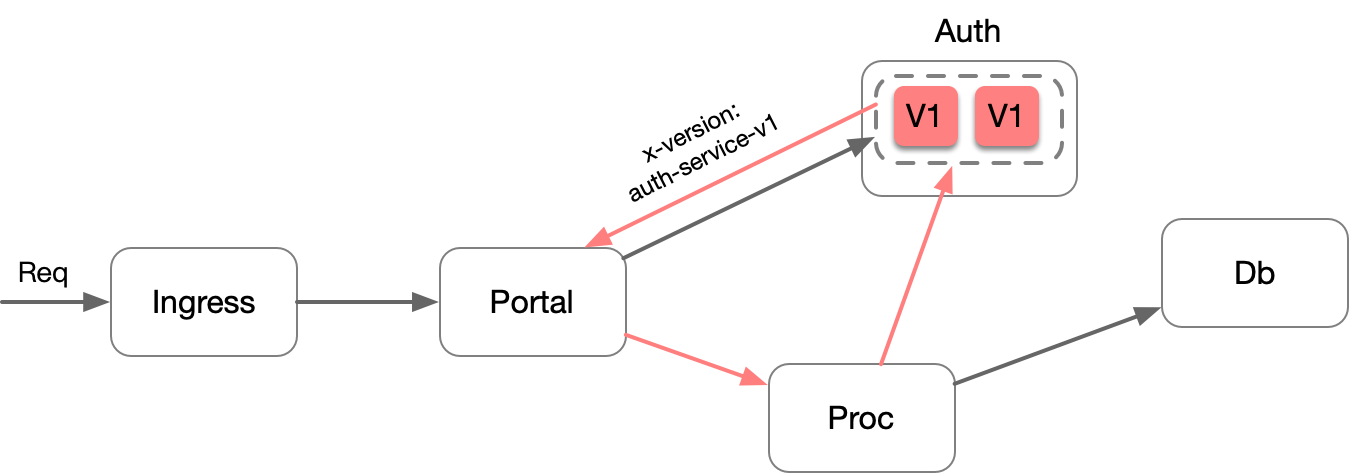
\includegraphics[height=4cm]{images/traffic_all_v1.png}
 \caption{流量全部发往v1}
 \label{fig:traffic_all_v1}
\end{figure}

在系统的运行过程中,当存在入站流量调用到auth-service时,Envoy容器执行拦截操作:一方面将流量转发往负责的服务实例,另一方面将此次调用所对应的traceid信息从头信息中提取出来并发送往TraceManager容器,TraceManager容器则将对应的traceid存到对应的TraceidSet中,该集合代表了当前所有调用过auth-service的分布式事务id;同时,当本次用户请求处理完成并返回Ingress Gateway时,Ingress Gateway实例内部会执行同样的添加操作,这里的TraceidSet则代表了当前已完成并返回的分布式事务id集合。
\begin{figure}[ht]
 \centering
 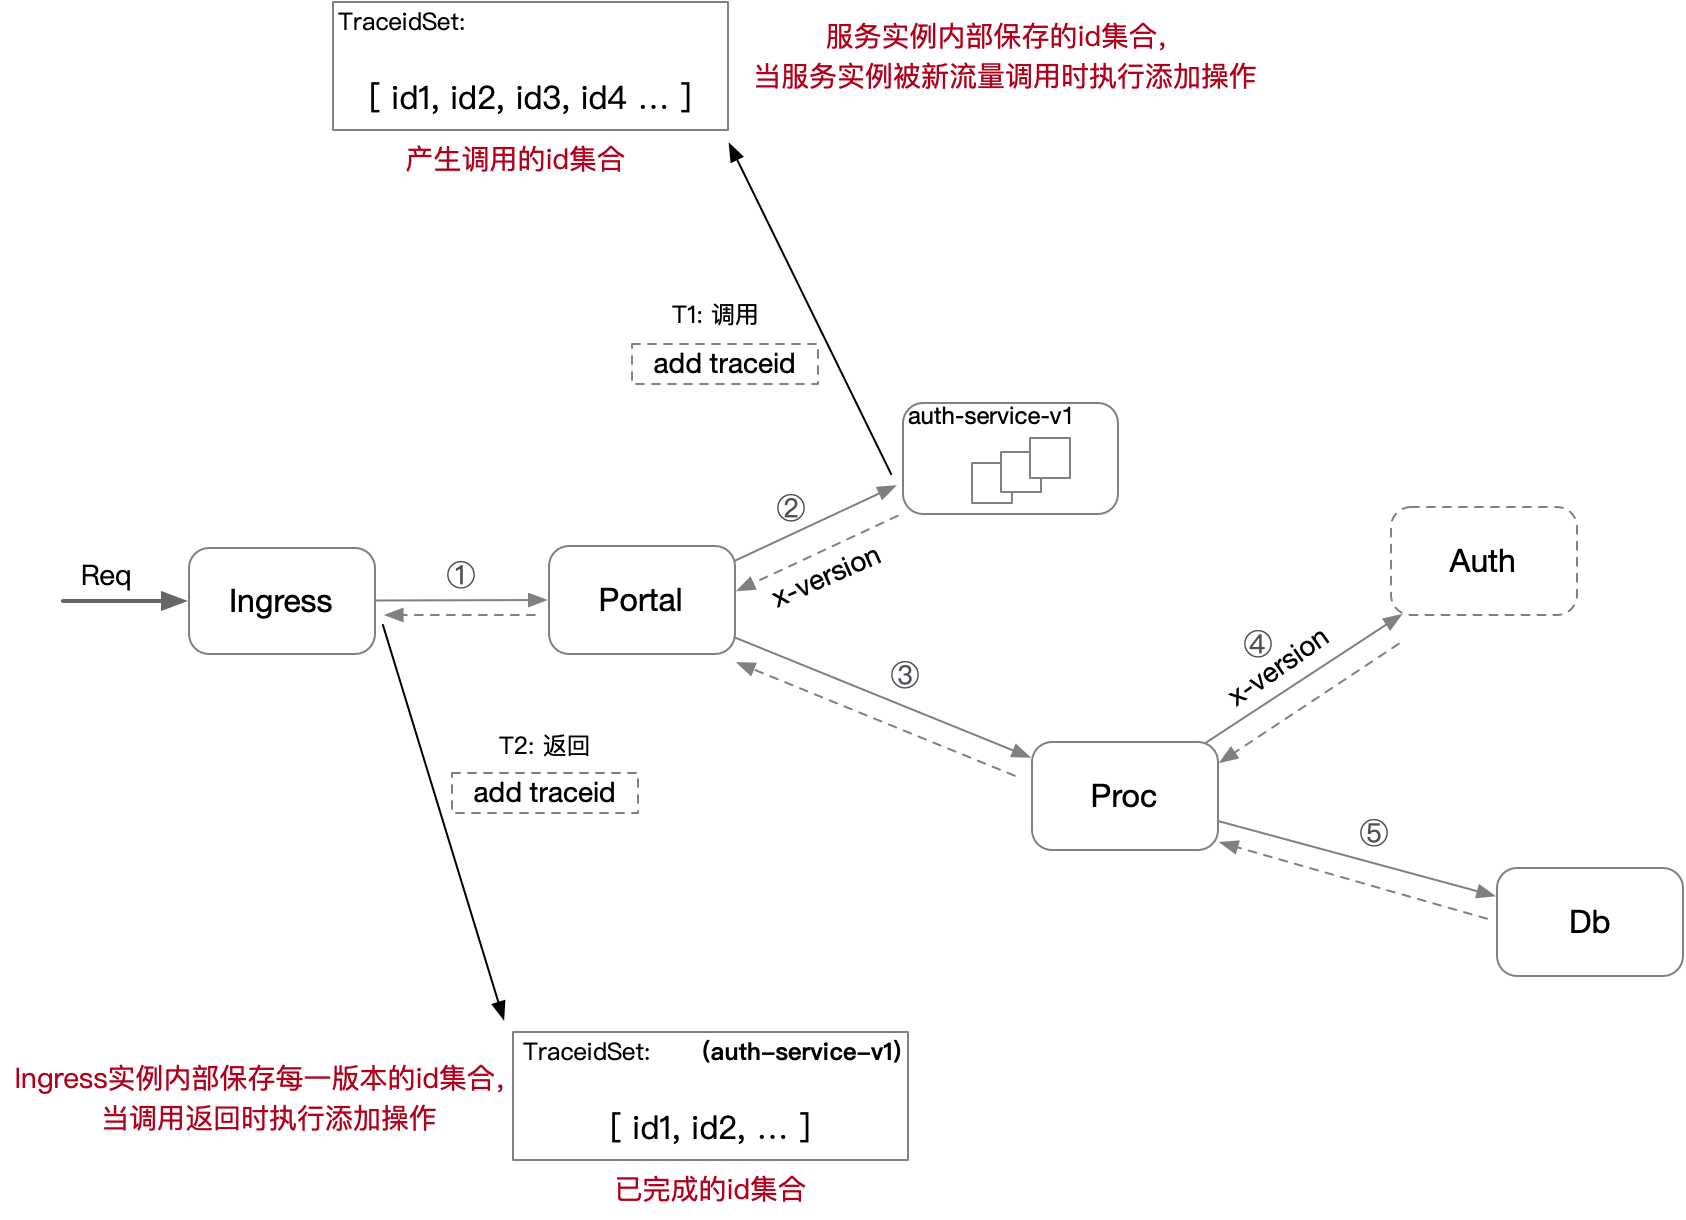
\includegraphics[height=10cm]{images/record_trace.png}
 \caption{事务记录}
 \label{fig:record_trace}
\end{figure}

\subsubsection{新版本上线}
当我们需要对auth-service进行更新时,首先需要将新版本的服务进行上线部署。与此同时,相关的路由规则和版本信息修改为:图\ref{fig:vs_default_v1}中共包含三个路由规则,依次进行匹配,第一条规则表示若请求流量中的头信息包含v1版本信息,则将该流量转发到v1版本中;第二条规则表示若请求流量中的头信息包含v2版本信息,则将该流量转发到v2版本中;若第一第二条规则均不满足,则应用第三条规则,将流量转发到v1版本中,同时添加对应的自定义头信息。图\ref{fig:dr_v1v2}则添加了新版本服务对应的标签定义。
\begin{figure}[htbp]
\centering
\begin{minipage}[t]{0.48\textwidth}
\centering
\centerline{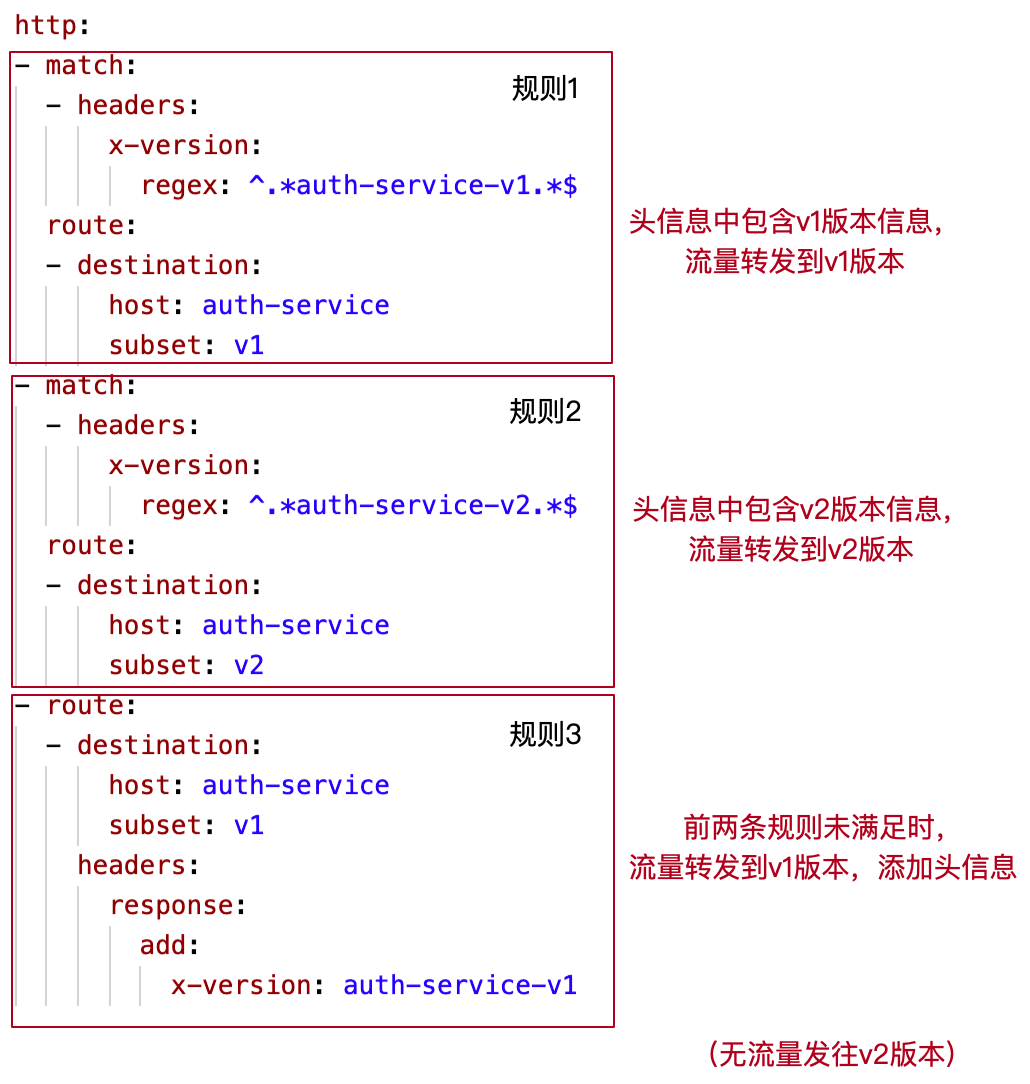
\includegraphics[width=7cm]{vs_default_v1.png}}
\caption{默认发往v1路由规则}
\label{fig:vs_default_v1}
\end{minipage}
\begin{minipage}[t]{0.48\textwidth}
\centering
\centerline{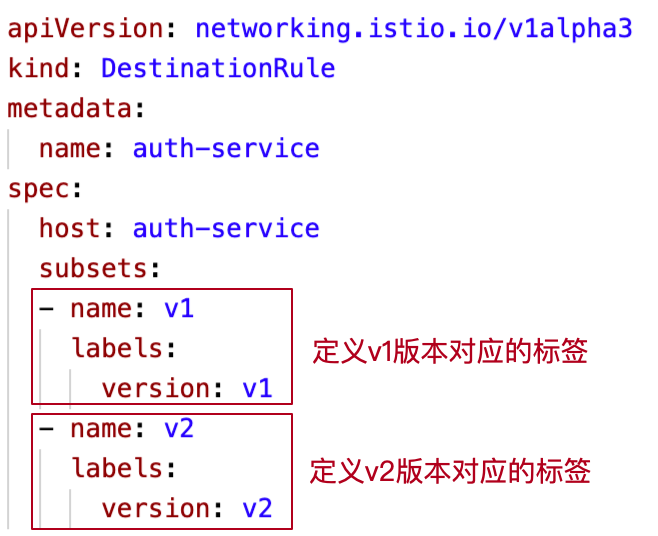
\includegraphics[width=6cm]{dr_v1v2.png}}
\caption{v1、v2版本规则}
\label{fig:dr_v1v2}
\end{minipage}
\end{figure}

此时,若某个分布式事务还未调用过auth-service,则请求的头信息中不包含相关的版本信息,依据第三条规则将流量转发往v1版本;若此分布式事务已调用过auth-service服务,则由于第三条规则的存在,其请求的头信息中必然包含了v1的版本信息,依据第一条规则同样将流量转发往v1版本。因此,虽然新版本的auth-service已完成上线部署,但还没有流量经过。对应的系统运行状态如图\ref{fig:traffic_default_v1}所示
\begin{figure}[ht]
 \centering
 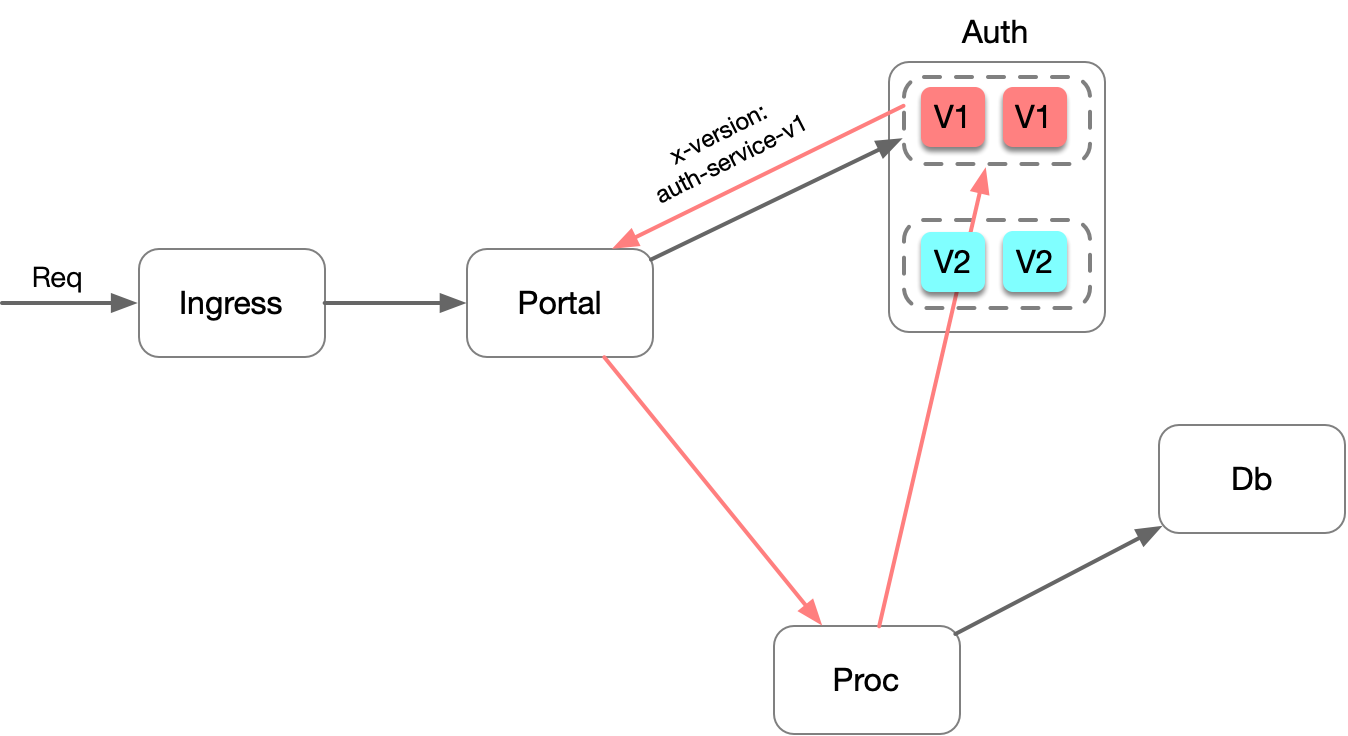
\includegraphics[height=5cm]{images/traffic_default_v1.png}
 \caption{流量默认发往v1}
 \label{fig:traffic_default_v1}
\end{figure}

\subsubsection{路由规则更新}\label{section:update_route}
待前一步骤的配置完成,我们接着对路由规则进行配置修改:如图\ref{fig:vs_default_v2}所示,前两条规则并未发生修改,依然是优先根据头信息中的相关内容来进行流量的转发。关键在于将第三条规则的默认流量转发从v1改为v2。

\begin{lemma}
进行第三步的路由规则更新,将默认的流量转发目标从v1改为v2,不影响任何分布式事务的版本一致性,无论该分布式事务处于系统运行中的哪个阶段。
\end{lemma}

\begin{proof}
对于任何一个分布式事务T,若T在运行的过程中还未调用过auth-service,则请求的头信息中不包含相关的版本信息,依据规则T将使用v2版本,不违背版本一致性;若T在过往子事务的运行过程中调用过auth-service,则请求的头信息中必然包含相关的版本信息,此时路由规则将进行相关的头信息版本匹配,并转发往同一版本的auth-service,保证了版本一致性;若T在将来的运行过程中不会再调用auth-service,同样不违背版本一致性。因此证明了进行第三步\ref{section:update_route}的路由规则更新,任何分布式事务T都满足版本一致性的要求。
\end{proof}

\begin{figure}[ht]
 \centering
 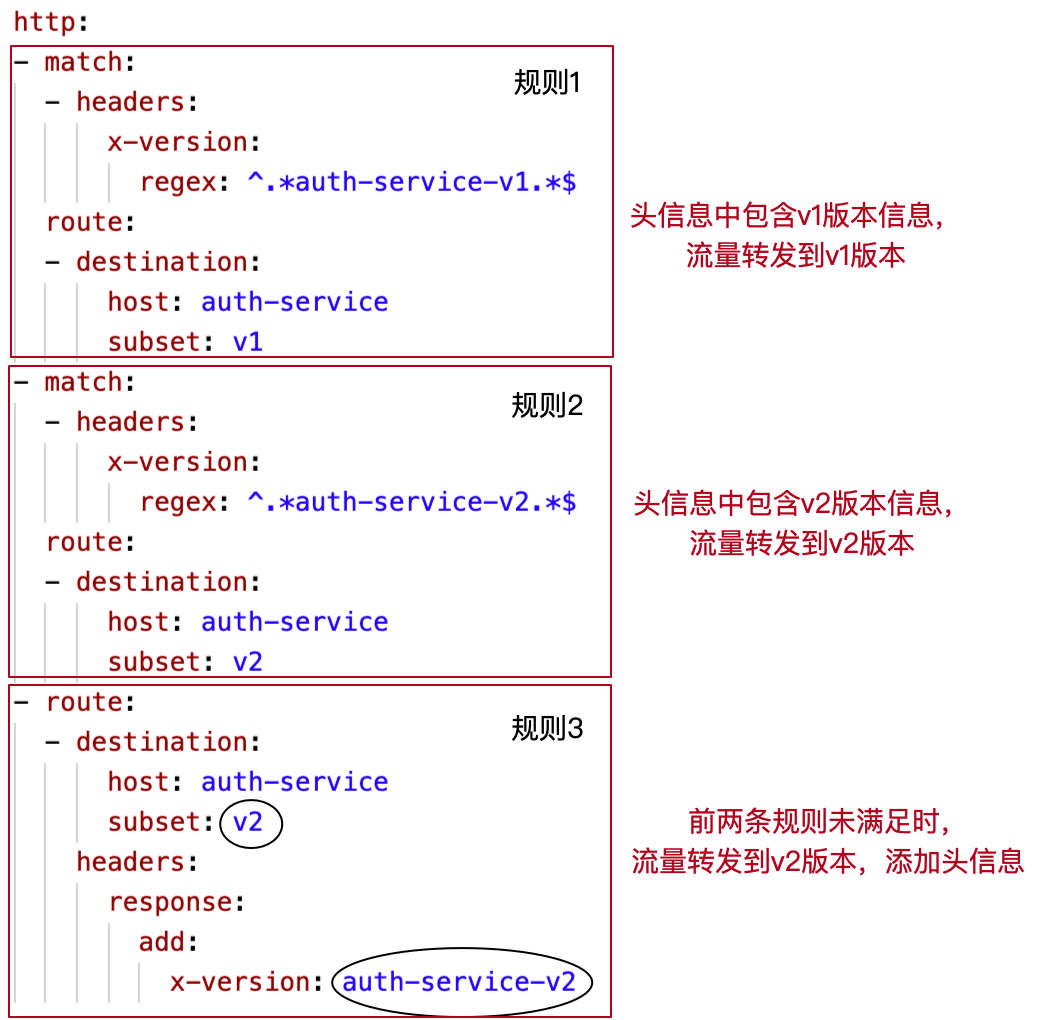
\includegraphics[height=8cm]{images/vs_default_v2.png}
 \caption{默认发往v2路由规则}
 \label{fig:vs_default_v2}
\end{figure}

更新完路由规则对应的系统运行状态如图\ref{fig:traffic_v1v2}所示,新产生的请求将发往新版本v2,运行中的请求则依据头信息内容进行匹配。
\begin{figure}[ht]
 \centering
 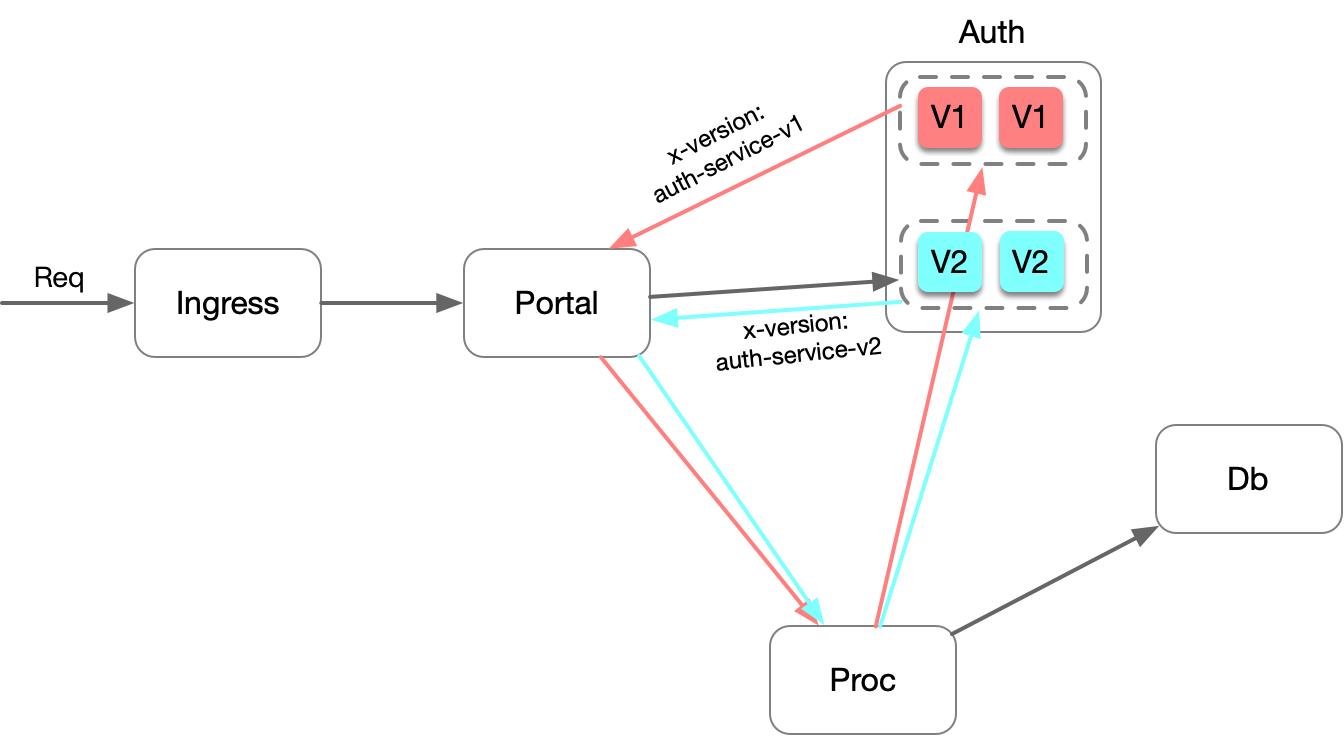
\includegraphics[height=5cm]{images/traffic_v1v2.png}
 \caption{新流量发往v2}
 \label{fig:traffic_v1v2}
\end{figure}

\subsubsection{旧版本撤销请求}
完成前述步骤后,我们便完成了新旧版本流量的正确导向,新产生的用户请求也可以及时地使用新版本的服务。进一步我们希望能够及时地对旧版本的服务实例进行撤销,避免其长时间地占用系统的资源。我们需要进行判断:何时旧版本的服务实例上的事务全部结束且不会再为其它事务提供服务?这时,便需要使用TraceManager容器中所保存的TraceidSet。具体实现包括以下步骤:
\begin{enumerate}
	\item 阻塞访问旧版本:当收到旧版本的撤销请求时,阻塞所有调用旧版本服务实例的新请求,即头信息中不存在对应版本信息的流量,同时直接返回503(Service Not Available)错误,在调用方侧执行重试机制,此时调用方将应用较新的路由规则,流量被转发到新版本的服务中。从而保证了不会再有新请求调用到旧版本服务实例,并且对TraceManager容器中保存的TraceidSet执行加锁,不再向其中添加traceid,此时TraceidSet保存了所有调用过旧版本服务实例的分布式事务id。流程如图\ref{fig:block_and_retry}所示;
	\begin{figure}[ht]
	 \centering
	 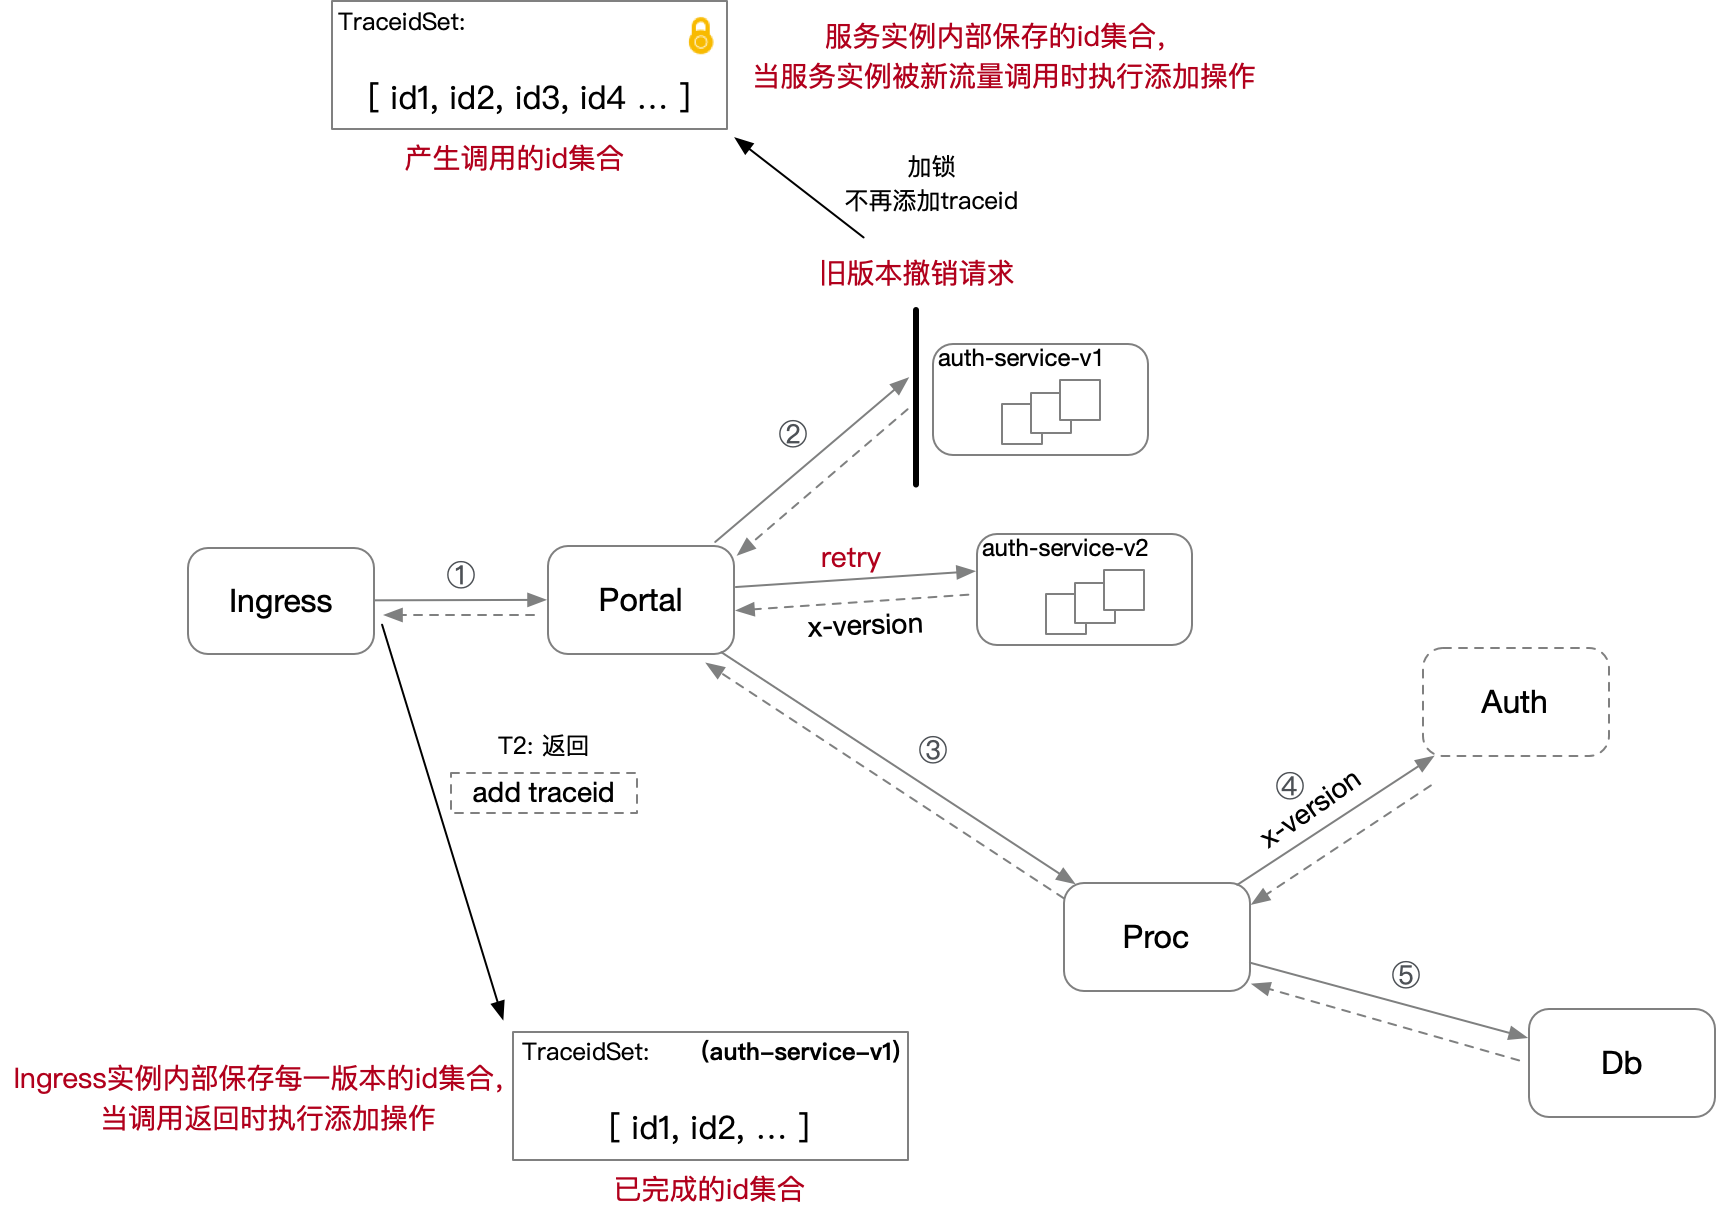
\includegraphics[height=10cm]{images/block_and_retry.png}
	 \caption{阻塞访问旧版本}
	 \label{fig:block_and_retry}
	\end{figure}

	\item 同步Traceid集合:将所有旧版本实例中所保存的TraceidSet发送至Ingress Gateway。Ingress Gateway此时暂时阻塞添加Traceid,将收到的TraceidSet和自己内部保存的TraceidSet进行同步,求得差集DiffSet。此差集便表示了所有调用过旧版本服务,但还未将运行结果返回给Ingress Gateway的分布式事务id集合。示例如图\ref{fig:sync_traceid}所示;
	\begin{figure}[ht]
	 \centering
	 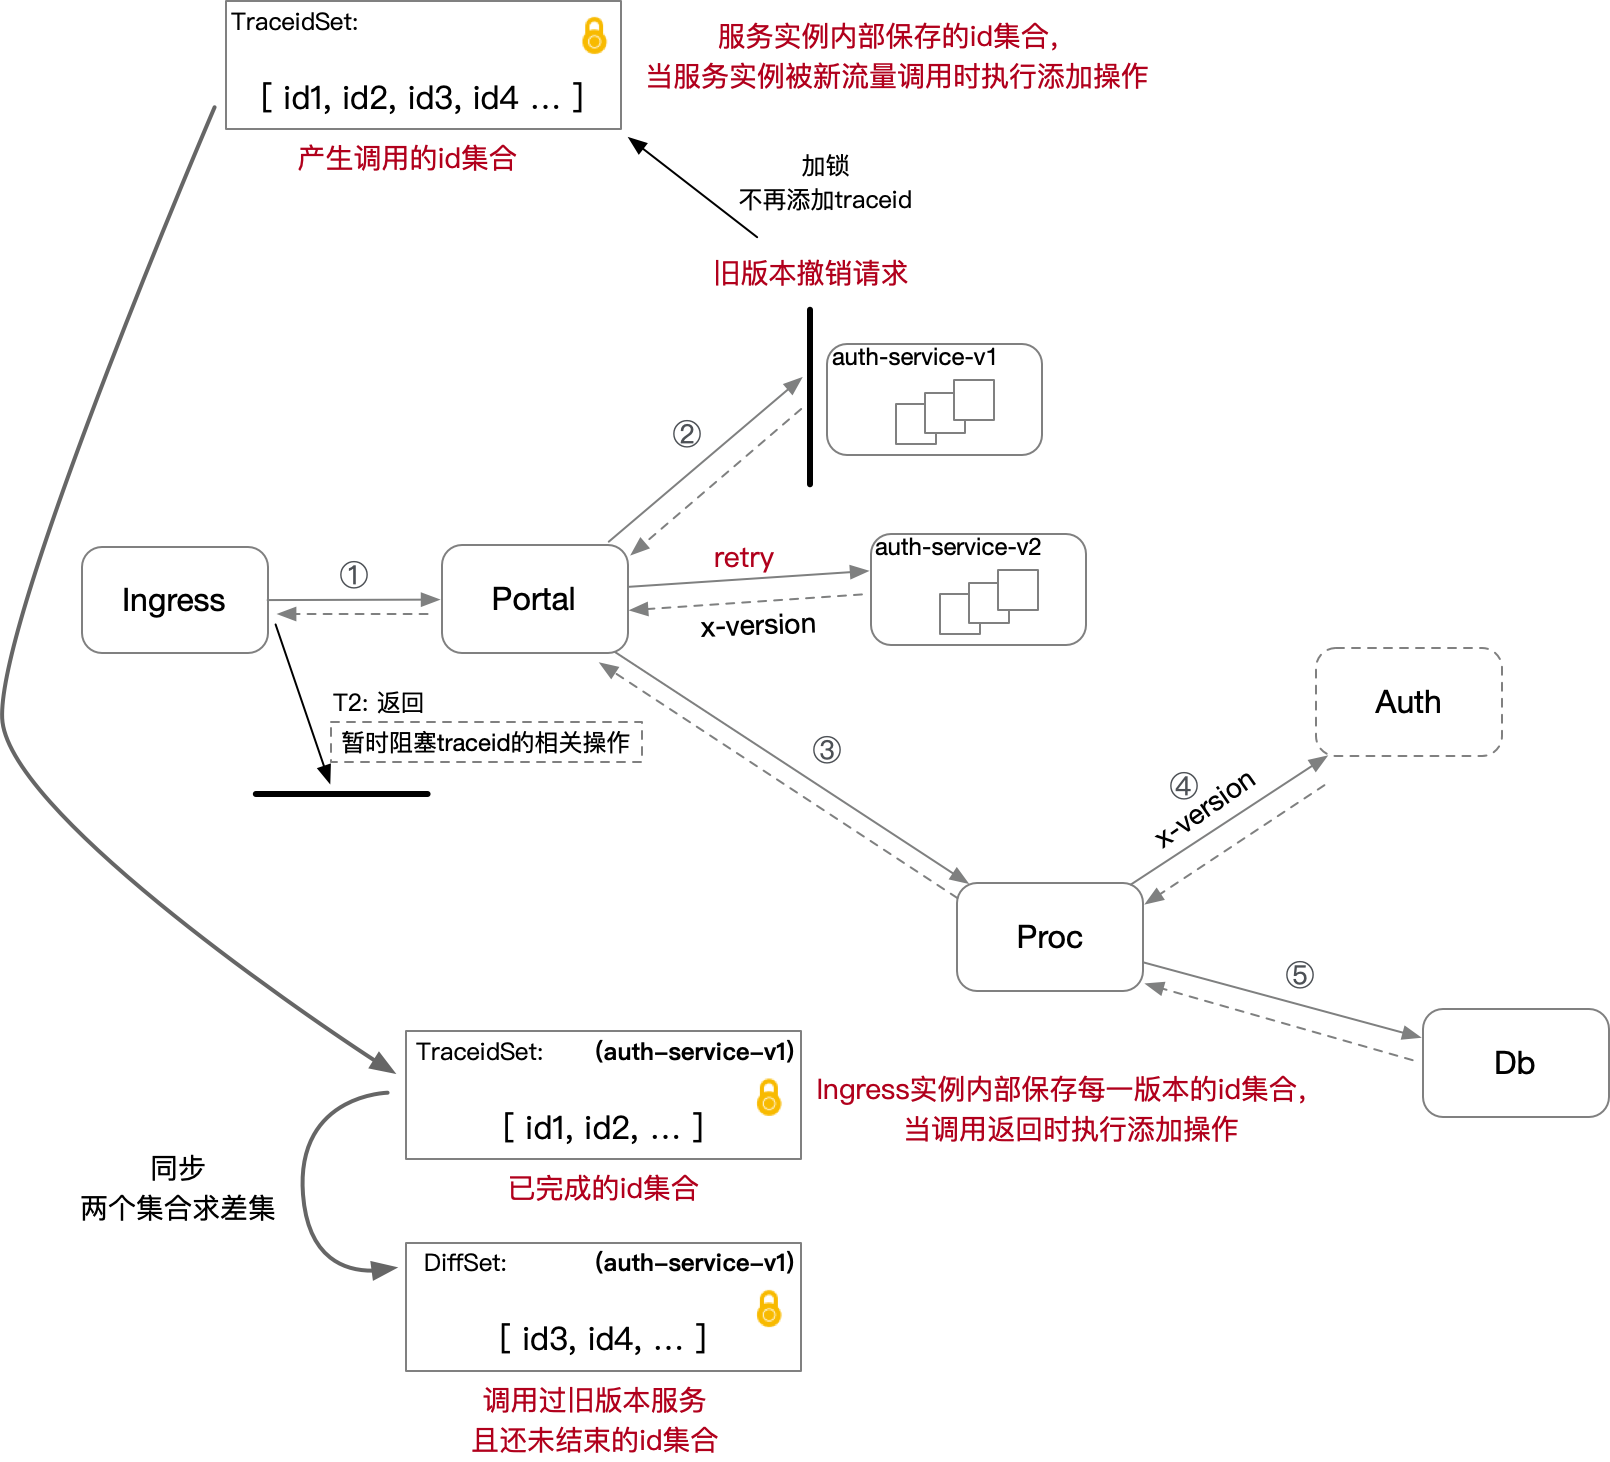
\includegraphics[height=10cm]{images/sync_traceid.png}
	 \caption{同步Traceid集合}
	 \label{fig:sync_traceid}
	\end{figure}

	\item 利用差集完成旧版本的撤销:在得到前一步骤的差集结果DiffSet后,不再阻塞Traceid的相关操作,对于收到的每一个Traceid,将其从DiffSet中删除,表示该分布式事务运行完成并返回结果。当差集DiffSet最终删除为空集时,我们便可以做出推断:所有已调用过旧版本服务的分布式事务均已返回结果,旧版本服务实例可被撤销。具体如图\ref{fig:wait_for_revoke}所示;
	\begin{figure}[ht]
	 \centering
	 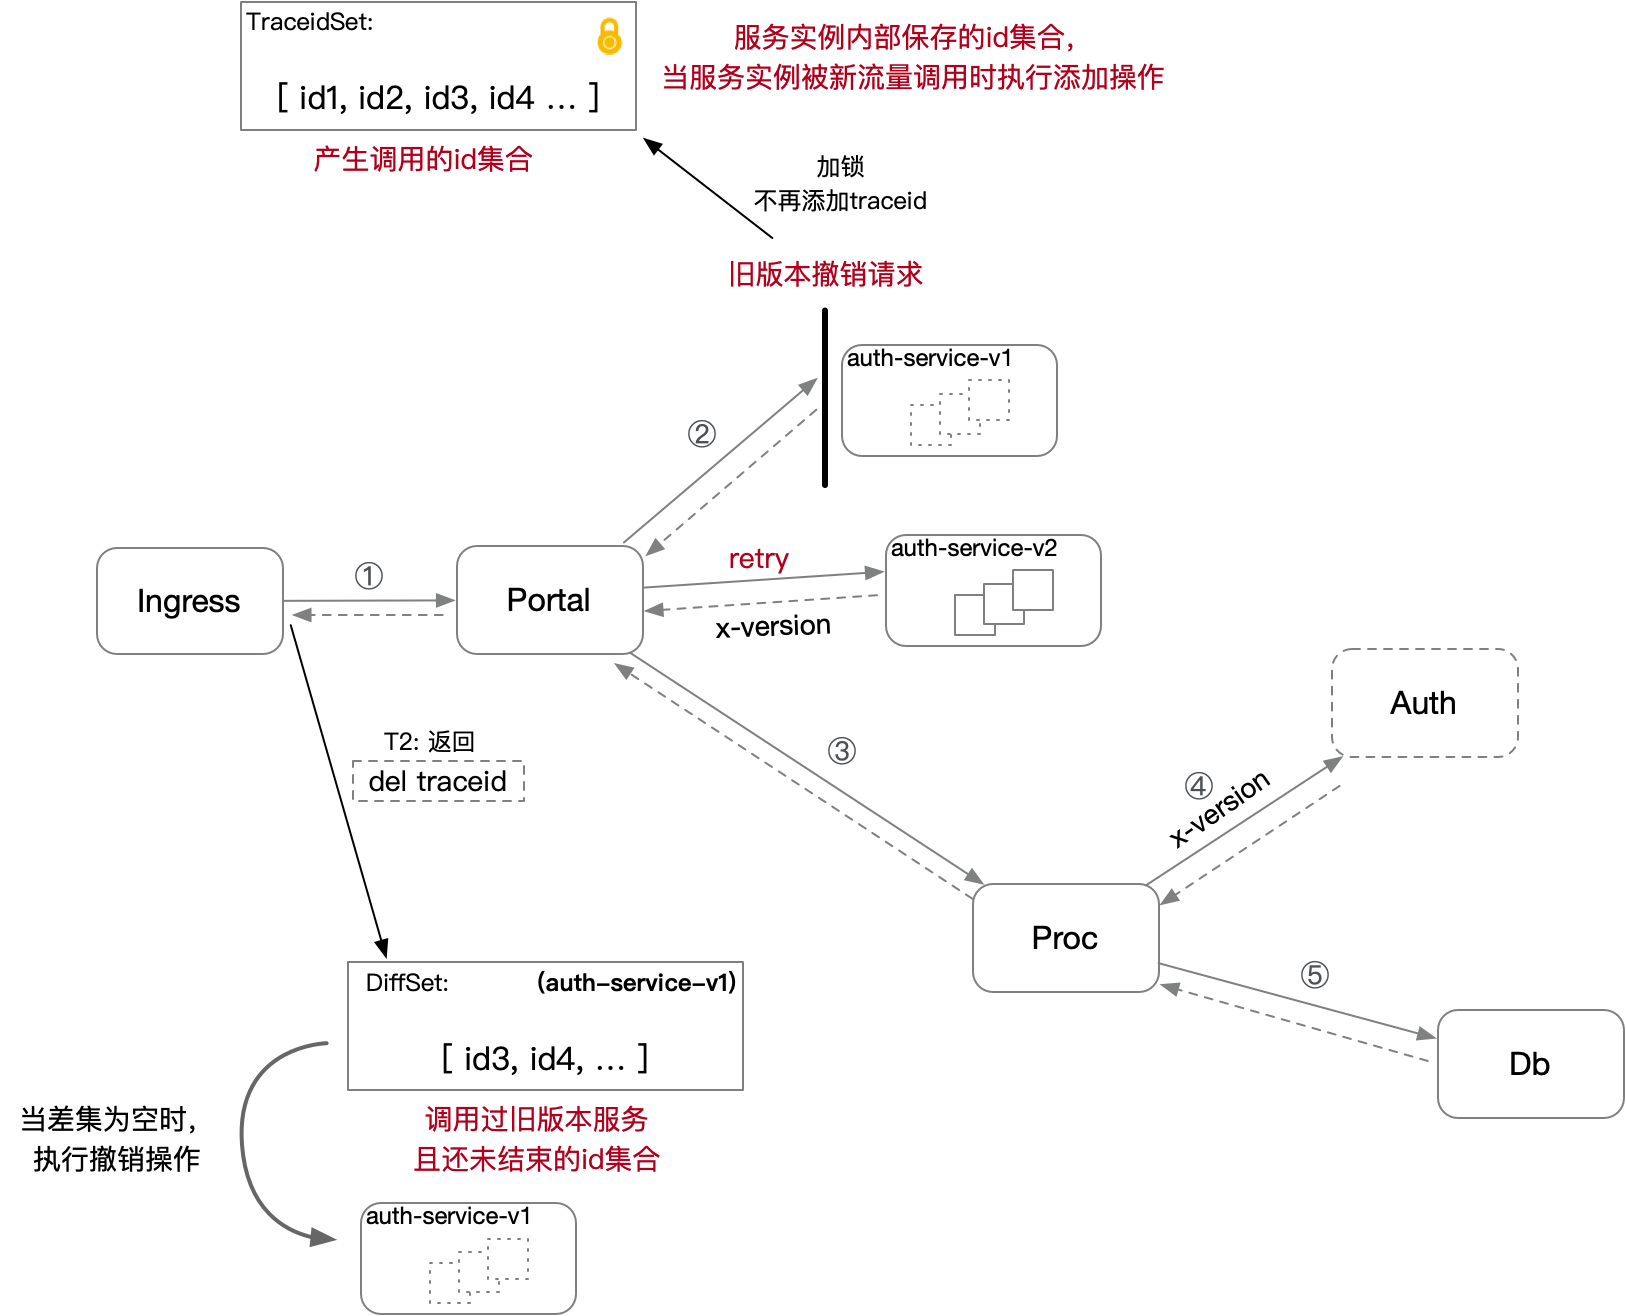
\includegraphics[height=10cm]{images/wait_for_revoke.png}
	 \caption{利用差集完成旧版本的撤销}
	 \label{fig:wait_for_revoke}
	\end{figure}
\end{enumerate}

\subsubsection{旧版本撤销与清理操作}
完成前述步骤后,我们就可以安全地撤销掉旧版本的所有服务实例,同时对相关的配置进行清理,还原成类似步骤1\ref{section:setup}中的初始状态,只是相关的版本从v1变更为v2,为下一次更新操作奠定基础。具体的路由规则、版本规则和系统运行状态分布如图\ref{fig:vs_all_v2}、\ref{fig:dr_v2}、\ref{fig:traffic_all_v2}所示
\begin{figure}[htbp]
\centering
\begin{minipage}[t]{0.48\textwidth}
\centering
\centerline{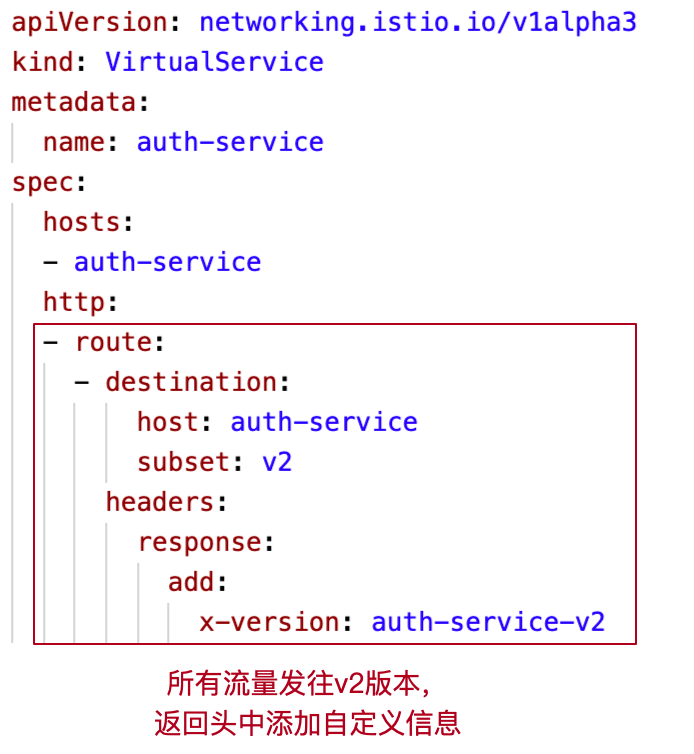
\includegraphics[width=7cm]{vs_all_v2.png}}
\caption{v2路由规则}
\label{fig:vs_all_v2}
\end{minipage}
\begin{minipage}[t]{0.48\textwidth}
\centering
\centerline{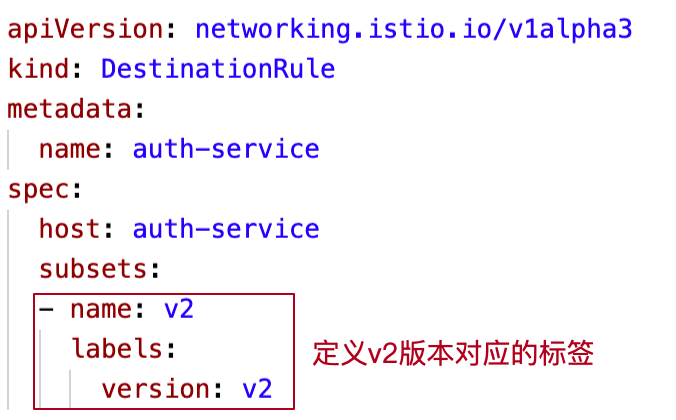
\includegraphics[width=6cm]{dr_v2.png}}
\caption{v2版本规则}
\label{fig:dr_v2}
\end{minipage}
\end{figure}
\begin{figure}[ht]
 \centering
 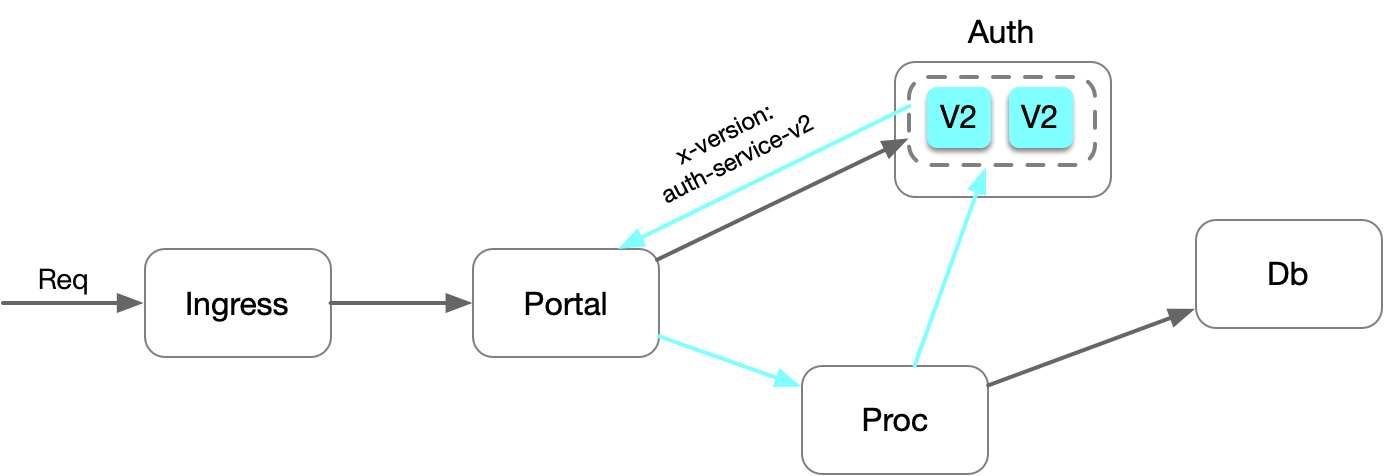
\includegraphics[height=5cm]{images/traffic_all_v2.png}
 \caption{流量全部发往v2}
 \label{fig:traffic_all_v2}
\end{figure}

\newpage
\section{人机物融合平台架构与技术集成} 

互联网的快速发展催生新技术与新业务的出现。软件从单纯的信息处理环节逐步成为了应用价值观的主要载体,并形成将人、计算机以及物理世界相连接的人机物融合软件新形态。人机物融合平台旨在人机物三元融合开放多变的环境下,灵活地协同管理各种自治的资源,支撑人机物融合应用系统的运行。

\subsection{总体的设计和结构}

人机物融合平台的运行环境基于当前最主流的容器化编排系统Kubernetes,在其上制定了一套人机物资源的描述规范,设计了一种消息驱动的人机物资源协作模型,构建了一套面向人机物融合的资源服务治理框架。

\subsection{人机物资源的描述与编排}
  实际的物理资源都要抽象成一种数据结构存储在系统中,系统同时要更新和维护它们。本软件平台通过Kubernetes CRD在系统中表示抽象资源,存储在etcd中,Kubernetes Controller负责维护它们,同步状态。
\subsubsection{人机物资源描述规范}
CRD是CustomResourceDefinition的简写,资源是kubernetes中的抽象概念,CRD是自定义的资源。

所有物理资源都要在系统中注册,且在系统中表达为Resource CRD,需要使用一些参数描述资源。这些参数告诉了Kubernetes平台如何去访问资源并维护资源的状态。首先,资源需要一个唯一的标识。其次,因为需要使用探针去采集资源的各项信息,需要包含探针程序的镜像地址和启动命令以及启动参数。

\begin{table}[!htbp]
\centering
\begin{tabular}{ccc}
  \toprule
  字段& 类型& 意义\\
  \midrule
  ResourceKind& enum& 资源类型,包括人、机器、服务\\
  Icon& string& 标识位置,用于在前端显示\\
  Description& map[string]string& 资源描述\\
  AccessMode& ResourceAccessMode& 访问方式,独占或者共享\\
  AliasName& string& 资源别名\\
  ProbeSpec& ProbeSpec& 探针属性\\
  ConnectorSpec& ConnectorSpec& 连接器属性\\
  \bottomrule
\end{tabular}
\caption{ResourceSpec}
\end{table}

\begin{table}[!htbp]
\centering
\begin{tabular}{ccc}
  \toprule
  字段& 类型& 意义\\
  \midrule
  Enabled& bool& 决定是否启用探针\\
  Image& string& 探针的镜像\\
  Args& []string& 探针的启动参数\\
  Patchers& []FieldPatcher& \\
  \bottomrule
\end{tabular}
\caption{ProbeSpec}
\end{table}

\begin{table}[!htbp]
\centering
\begin{tabular}{ccc}
  \toprule
  字段& 类型& 意义\\
  \midrule
  Source& HTTPActionSpec&  \\
  Setters& []FieldSetter&  \\
  \bottomrule
\end{tabular}
\caption{FieldPatcher}
\end{table}

\begin{table}[!htbp]
\centering
\begin{tabular}{ccc}
  \toprule
  字段& 类型& 意义\\
  \midrule
  Parser& string& 解析器\\
  Type& string& 类型\\
  Target& HTTPActionSpec& \\
  \bottomrule
\end{tabular}
\caption{FieldSetter}
\end{table}

\begin{table}[!htbp]
\centering
\begin{tabular}{ccc}
  \toprule
  字段& 类型& 意义\\
  \midrule
  Action& string& 接口名称\\
  URL& string& 接口url\\
  Query& map[string]string& 对接口的查询参数\\
  Headers& map[string]string& 请求头\\
  \bottomrule
\end{tabular}
\caption{HTTPActionSpec}
\end{table}

\begin{table}[!htbp]
\centering
\begin{tabular}{ccc}
  \toprule
  字段& 类型& 意义\\
  \midrule
  Image& string& 连接器镜像\\
  Args& []string& 连接器的启动参数\\
  ListenPort& int32& 连接器监听的端口\\
  \bottomrule
\end{tabular}
\caption{ConnectorSpec}
\end{table}

\begin{table}[!htbp]
\centering
\begin{tabular}{ccc}
  \toprule
  字段& 类型& 意义\\
  \midrule
  Phase& enum& 状态(包括Pending、Running、Failed)\\
  ProbePhase& enum& 探针状态(包括NotReady、Pending、Synchronous和Failed)\\
  Bound& bool& 是否已经被绑定使用\\
  CreateTime& *metav1.Time& 创建时间\\
  StartTime& *metav1.Time& 各个组件都启动的时间\\
  \bottomrule
\end{tabular}
\caption{ResourceStatus}
\end{table}

\subsubsection{人机物资源的运行时编排}

Linux容器技术能够对应用及其整个运行时环境(包括全部所需文件)一起进行打包或隔离。从而让开发者可以在不同环境(如开发、测试和生产等环境)之间轻松迁移应用,同时还可保留应用的全部功能。

容器是虚拟化的主要形式之一,相比于虚拟机需要虚拟化基础硬件,每个虚拟机都运行一个操作系统,容器共享主机OS,因此它们不需要启动 OS 或加载库。这使得容器更加高效和轻量。容器化应用程序可以在几秒钟内启动,与 VM 方案相比,应用程序的更多实例可以适应计算机。共享 OS 方法具有额外的好处,即减少维护(如修补和更新)开销。

Kubernetes提供了生产级容器编排服务,它是一种可自动实施 Linux 容器操作的开源平台。它可以帮助用户省去应用容器化过程的许多手动部署和扩展操作。Kubernetes 可为用户提供一个便捷有效的平台,让用户可以在物理机或虚拟机集群上调用和运行容器。Kubernetes 架构将集群分为不同的组件,这些组件要协同工作来维护集群的预期状态。

Kubernetes Operator 是一种封装、部署和管理 Kubernetes 应用的方法。Operator 是使用自定义资源(CR)管理应用及其组件的自定义 Kubernetes 控制器。高级配置和设置由用户在 CR 中提供。Kubernetes Operator 基于嵌入在 Operator 逻辑中的最佳实践将高级指令转换为低级操作。自定义资源是 Kubernetes 中的 API 扩展机制。自定义资源定义(CRD)会明确 CR 并列出 Operator 用户可用的所有配置。 Kubernetes Operator 监视 CR 类型并采取特定于应用的操作,确保当前状态与该资源的理想状态相符。

我们使用Operator的形式在Kubernetes中部署人机物融合平台。
Resource CRD由Resource Controller管理,控制器监控资源的状态,当监测资源的增删改事件时就会生成一个包含相关资源名称的request塞入工作队列,Reconcile方法每隔很短的一段时间被调用一次,从工作队列中取出一个request作为参数进行处理。

Reconcile首先根据request中包裹的资源名称和命名空间找到Resource的实例,如果是删除事件什么都不需要做,增改事件则会判断是否需要新建、更新、删除包含探针和连接器的Deployment资源以及Service资源。

控制器的实际工作就是把Resource CRD翻译成Kubernetes中的原生资源,Deployment会负责生产实际的Pod来运行Probe和Connector容器,Service用于暴露Connector,让其他的应用可以访问它。

\subsection{消息驱动的人机物资源协作模型}
\subsubsection{资源状态的同步}
\subsubsection{资源代理服务(TC)}
\paragraph{资源代理描述}
资源代理在我们的平台中是以微服务的形式描述现实世界中资源的一些基本信息和它具有的能力,资源代理主要分为两类:智能设备和人。资源代理的基本信息除了包括id,品牌和它的一些基本属性之外,还包括它的时空属性信息;资源代理的能力实际上表示为\textbf{Restful API}定义的功能接口。目前我们采用传统的\textbf{MVC}架构,在\textbf{Spring Boot}框架上构建我们的资源代理。
\paragraph{资源代理实现}
具体实现方面,资源代理在我们的平台上是一个一个的\textbf{Spring Boot}微服务,资源代理的实现需要探针的配合,下面分别描述智能设备和人的资源代理的实现方式。
\begin{itemize}
 \item{\textbf{智能设备}}\\
 智能设备的资源代理相对固定,因为智能设备的功能是相对固定的,所以当资源代理部署完成之后,不需要对它的属性和功能接口进行大的修改。以空气净化器为例来介绍资源代理的实现。首先我们需要将空气净化器连接到\textbf{Home Assistant}这样的智能设备管理平台上,这样开发人员就可以从\textbf{Home Assistant}上获得空气净化器的属性信息和操控接口,相应地,在空气净化器的资源代理中,一方面,开发人员对空气净化器进行建模,将空气净化器的属性信息和时空属性加入元模型,并提供相应的修改查询接口给\textbf{探针}调用,另一方面开发人员需要封装\textbf{Home Assistant}提供的操纵接口,生成对应的\textbf{Restful API},使得用户可以通过\textbf{Restful API},借助\textbf{Home Assistant}来远程操控空气净化器。
 \begin{lstlisting}
    %   @PostMapping("/turnon")
        @Accessible("true")
        public String turnOnAirPurifier(){
           RestTemplate restTemplate = new RestTemplate();
           String url = "http://192.168.31.143:8123/api/services/fan/turn_on";
           HttpHeaders headers = new HttpHeaders();
           headers.add("Authorization","xxxxx");
           headers.setContentType(MediaType.APPLICATION_JSON);
           JSONObject jsonObject = new JSONObject();
           jsonObject.put("entity_id","fan.xiaomi_miio_device");
           HttpEntity<String> request = new HttpEntity<>(jsonObject.toString(),headers);
           return restTemplate.postForObject(url,request,String.class);
       }
    \end{lstlisting}
    \item{\textbf{人}}\\
    人的资源代理和智能设备的资源代理在实现方面有一些区别,人的资源代理描述了在某个具体场景下该人所具有的能力,所以随着人的活动,他的资源代理会不断更新。举例来说,当人进入一个只有空气净化器的房间时,现实世界中的人就增加了一个使用空气净化器的能力,在这个场景下,人的资源代理就会增加操控空气净化器的接口。当这个人从房间离开,进入一个有咖啡机的房间,那么现实世界中的人会失去使用空气净化器的能力,增加使用咖啡机的能力,相应地,人的资源代理也会相应更新,删除操控空气净化器的接口,增加操控咖啡机的接口。
\end{itemize}

\subsubsection{消息队列(TC)}

\subsection{面向人机物融合的资源服务治理框架}
\subsubsection{人机物融合场景下的服务路由(TC)}
\subsubsection{资源服务的动态更新(WDY)}

\section{动态更新系统实现}\label{section:MsDymEvo}

\subsection{基本设计概念和结构}

\subsection{项目管理器}
\subsubsection{模块描述}
项目团队中通常包括开发与运营团队,开发团队主要负责开发、测试、推送关键的业务逻辑代码,而运营团队则负责代码的部署、系统的维护等相关的运维工作。两个团队的工作需要密切的联系,但工作内容又泾渭分明。因此,本项目通过引入代码管理器作为开发团队和运营团队的中间处理器,接管双向请求的同时进行进一步的封装和屏蔽,较大程度的减少了侵入性,为两个团队之间的沟通架设好桥梁,使得两个团队可以快速的进行信息的交互,减少了两个团队之间沟通的时间成本,为整个应用系统之后的快速部署与更新迭代提供了保障。
\subsubsection{功能}
在代码管理器中,首先需要引入如下的概念:
\theoremstyle{definition}
\begin{definition}[\textbf{manifest}]
\label{definition:manifest}
manifest包含project下所有service的git仓库和当前运行版本号。
\end{definition}

\theoremstyle{definition}
\begin{definition}[\textbf{execResult}]
\label{definition:execResult}
execResult表示后台执行反馈,如succeeded/exception log等。
\end{definition}
代码管理器作为开发团队和运营团队的中间处理器,主要具备以下的功能:
\begin{itemize}
	\item{创建项目
	\begin{itemize}
	\item 输入:manifest
	\item 输出:execResult
	\item 描述:根据输入manifest, 创建gitlab group, 将manifest写入group description,并将manifest中指定的服务仓库添加到gitlab group shared projects, 目前每个仓库需为现有gitlab仓库
	\end{itemize}}
\end{itemize}

\subsection{构建管理器}

\subsection{更新控制器}

\subsection{运行说明}

% -----------------------------------Appendix----------------------------------------
% -----------------------------------REFERENCE----------------------------------------
\end{document}

